%% BioMed_Central_Tex_Template_v1.06
%%                                      %
%  bmc_article.tex            ver: 1.06 %
%                                       %

%%IMPORTANT: do not delete the first line of this template
%%It must be present to enable the BMC Submission system to
%%recognise this template!!

%%%%%%%%%%%%%%%%%%%%%%%%%%%%%%%%%%%%%%%%%
%%                                     %%
%%  LaTeX template for BioMed Central  %%
%%     journal article submissions     %%
%%                                     %%
%%          <8 June 2012>              %%
%%                                     %%
%%                                     %%
%%%%%%%%%%%%%%%%%%%%%%%%%%%%%%%%%%%%%%%%%


%%%%%%%%%%%%%%%%%%%%%%%%%%%%%%%%%%%%%%%%%%%%%%%%%%%%%%%%%%%%%%%%%%%%%
%%                                                                 %%
%% For instructions on how to fill out this Tex template           %%
%% document please refer to Readme.html and the instructions for   %%
%% authors page on the biomed central website                      %%
%% http://www.biomedcentral.com/info/authors/                      %%
%%                                                                 %%
%% Please do not use \input{...} to include other tex files.       %%
%% Submit your LaTeX manuscript as one .tex document.              %%
%%                                                                 %%
%% All additional figures and files should be attached             %%
%% separately and not embedded in the \TeX\ document itself.       %%
%%                                                                 %%
%% BioMed Central currently use the MikTex distribution of         %%
%% TeX for Windows) of TeX and LaTeX.  This is available from      %%
%% http://www.miktex.org                                           %%
%%                                                                 %%
%%%%%%%%%%%%%%%%%%%%%%%%%%%%%%%%%%%%%%%%%%%%%%%%%%%%%%%%%%%%%%%%%%%%%

%%% additional documentclass options:
%  [doublespacing]
%  [linenumbers]   - put the line numbers on margins

%%% loading packages, author definitions

%\documentclass[twocolumn]{bmcart}
% uncomment this for twocolumn layout and comment line below
\documentclass{bmcart}

%%% Load packages
%\usepackage{amsthm,amsmath}
%\RequirePackage{natbib}
\RequirePackage{hyperref}
% \usepackage{etoolbox}
\usepackage[utf8x]{inputenc} %unicode support
\usepackage{graphicx}
\usepackage{tikz}
\usepackage{amsmath}
\usepackage{listings}
\usepackage{bera}
\usepackage{multirow}
\usepackage{fancyvrb}
\usepackage{soul}
%\usepackage[applemac]{inputenc} %applemac support if unicode package fails
%\usepackage[latin1]{inputenc} %UNIX support if unicode package fails

%%%%%%%%%%%%%%%%%%%%%%%%%%%%%%%%%%%%%%%%%%%%%%%%%
%%                                             %%
%%  If you wish to display your graphics for   %%
%%  your own use using includegraphic or       %%
%%  includegraphics, then comment out the      %%
%%  following two lines of code.               %%
%%  NB: These line *must* be included when     %%
%%  submitting to BMC.                         %%
%%  All figure files must be submitted as      %%
%%  separate graphics through the BMC          %%
%%  submission process, not included in the    %%
%%  submitted article.                         %%
%%                                             %%
%%%%%%%%%%%%%%%%%%%%%%%%%%%%%%%%%%%%%%%%%%%%%%%%%

%\def\includegraphic{}
%\def\includegraphics{}
\errorcontextlines 10000

% \makeatletter
% \patchcmd{\@addmarginpar}{\ifodd\c@page}{\ifodd\c@page\@tempcnta\m@ne}{}{}
% \makeatother
% \reversemarginpar

%%% Put your definitions there:
\startlocaldefs
  \newcommand{\comment}[2]{\hspace{0in}#2}
  \lstdefinelanguage{json}{
      basicstyle=\normalfont\ttfamily,
      numbersep=8pt,
      showstringspaces=false,
      breaklines=true,
      frame=lines,
      backgroundcolor=\color{white},
  }
\endlocaldefs


%%% Begin ...
\begin{document}

%%% Start of article front matter
\begin{frontmatter}

\begin{fmbox}
\dochead{Software}

%%%%%%%%%%%%%%%%%%%%%%%%%%%%%%%%%%%%%%%%%%%%%%
%%                                          %%
%% Enter the title of your article here     %%
%%                                          %%
%%%%%%%%%%%%%%%%%%%%%%%%%%%%%%%%%%%%%%%%%%%%%%

\title{``gnparser'':  A powerful semantic parser for scientific names based on
  parsing expression grammars}


%%%%%%%%%%%%%%%%%%%%%%%%%%%%%%%%%%%%%%%%%%%%%%
%%                                          %%
%% Enter the authors here                   %%
%%                                          %%
%% Specify information, if available,       %%
%% in the form:                             %%
%%   <key>={<id1>,<id2>}                    %%
%%   <key>=                                 %%
%% Comment or delete the keys which are     %%
%% not used. Repeat \author command as much %%
%% as required.                             %%
%%                                          %%
%%%%%%%%%%%%%%%%%%%%%%%%%%%%%%%%%%%%%%%%%%%%%%

\author[
   addressref={aff1},
   corref={aff1},                       % id of corresponding address, if any
   email={mozzheri@illinois.edu}
]{\inits{DYM}\fnm{Dmitry Y.} \snm{Mozzherin}}
\author[                  % id's of addresses, e.g. {aff1,aff2}
   addressref={aff2},
   noteref={n1},% id's of article notes, if any
   email={alexander@myltsev.com}   % email address
]{\inits{AAM}\fnm{Alexander A.} \snm{Myltsev}}
\author[
   addressref={aff3},
   email={dpatterson.mbl@gmail.com}
]{\inits{DJP}\fnm{David J.} \snm{Patterson}}

%%%%%%%%%%%%%%%%%%%%%%%%%%%%%%%%%%%%%%%%%%%%%%
%%                                          %%
%% Enter the authors' addresses here        %%
%%                                          %%
%% Repeat \address commands as much as      %%
%% required.                                %%
%%                                          %%
%%%%%%%%%%%%%%%%%%%%%%%%%%%%%%%%%%%%%%%%%%%%%%

\address[id=aff1]{                     % unique id
  \orgname{University of Illinois},    % university, etc
  \street{1816 South Oak St.},         %
  \city{Champaign},                    % city
  \state{IL},
  \postcode{61820},
  \cny{US}                             % country
}

\address[id=aff2]{                     % unique id
  \orgname{IP Myltsev},                % university, etc
  \street{Kaslinskaya St.},            %
  \city{Chelyabinsk},                  % city
  \state{},
  \postcode{454084},
  \cny{Russia}                         % country
}

\address[id=aff3]{                     % unique id
  \orgname{University of Sydney},      % university, etc
  \city{Sydney},                       % city
  \cny{Australia}                      % country
}

%%%%%%%%%%%%%%%%%%%%%%%%%%%%%%%%%%%%%%%%%%%%%%
%%                                          %%
%% Enter short notes here                   %%
%%                                          %%
%% Short notes will be after addresses      %%
%% on first page.                           %%
%%                                          %%
%%%%%%%%%%%%%%%%%%%%%%%%%%%%%%%%%%%%%%%%%%%%%%

\begin{artnotes}
%\note{Sample of title note}     % note to the article
\note[id=n1]{Equal contributor} % note, connected to author
\end{artnotes}

\end{fmbox}% comment this for two column layout

%%%%%%%%%%%%%%%%%%%%%%%%%%%%%%%%%%%%%%%%%%%%%%
%%                                          %%
%% The Abstract begins here                 %%
%%                                          %%
%% Please refer to the Instructions for     %%
%% authors on http://www.biomedcentral.com  %%
%% and include the section headings         %%
%% accordingly for your article type.       %%
%%                                          %%
%%%%%%%%%%%%%%%%%%%%%%%%%%%%%%%%%%%%%%%%%%%%%%

\begin{abstractbox}

\begin{abstract} % abstract

  \parttitle{Background} We will be able to investigate biology in new and
  different ways and on grander scales when we can integrate biological data
  from multiple sources. An obvious solution lies in using the scientific names
  of organisms as metadata. There are impediments to this because there may be
  many names for a taxon, or one name may apply to different taxa.  Names are
  represented by name-strings (a combination of characters, spaces and
  punctuation that represent the name). Within these, the same names may be
  spelled differently, be abbreviated, be annotated, or include or exclude
  authors of names and dates of establishment. We can minimize mismatches
  caused by such differences if we divide the name-strings into their component
  parts and establish the roles of each part that is, subject them to 'semantic
  parsing'. Once done, we can match entries on the most commonly used elements
  of names and/or set aside the elements that differ.

  \parttitle{Results} We introduce Global Names Parser (\textit{gnparser}), a
  tool based on the Parsing Expression Grammar algorithm. The parser is applied
  to scientific name-strings of any complexity. It assigns a semantic meaning
  (such as genus name, species epithet, annotation, rank, year of publication,
  names of authors, annotations, etc.) to all elements. Global Names Parser is
  written in Scala, a Java Virtual Machine language. It performs with $\approx
  99\%$ accuracy and processes 21.4 million name-strings/hour per CPU (73.4
  million names/hour per 4 CPUs). The \textit{gnparser} library is compatible
  with Scala, Java, R, Jython, and JRuby. The parser can be used as a command
  line application, socket server, web-app or RESTful http-service. It is
  released under an Open Source MIT license.

  \parttitle{Conclusions} Global Names Parser (\textit{gnparser}) is a fast,
  high precision tool for bioinformaticians and biologists working with large
  numbers of scientific names. It can replace expensive and error-prone manual
  parsing and standardization of scientific names in many situations and
  quickly increases the interoperability of distributed biological information.

\end{abstract}

%%%%%%%%%%%%%%%%%%%%%%%%%%%%%%%%%%%%%%%%%%%%%%
%%                                          %%
%% The keywords begin here                  %%
%%                                          %%
%% Put each keyword in separate \kwd{}.     %%
%%                                          %%
%%%%%%%%%%%%%%%%%%%%%%%%%%%%%%%%%%%%%%%%%%%%%%

\begin{keyword}
\kwd{biodiversity}
\kwd{biodiversity informatics}
\kwd{scientific name}
\kwd{parser}
\kwd{semantic parser}
\end{keyword}

% MSC classifications codes, if any
%\begin{keyword}[class=AMS]
%\kwd[Primary ]{}
%\kwd{}
%\kwd[; secondary ]{}
%\end{keyword}

\end{abstractbox}
%
%\end{fmbox}% uncomment this for twcolumn layout

\end{frontmatter}

%%%%%%%%%%%%%%%%%%%%%%%%%%%%%%%%%%%%%%%%%%%%%%
%%                                          %%
%% The Main Body begins here                %%
%%                                          %%
%% Please refer to the instructions for     %%
%% authors on:                              %%
%% http://www.biomedcentral.com/info/authors%%
%% and include the section headings         %%
%% accordingly for your article type.       %%
%%                                          %%
%% See the Results and Discussion section   %%
%% for details on how to create sub-sections%%
%%                                          %%
%% use \cite{...} to cite references        %%
%%  \cite{koon} and                         %%
%%  \cite{oreg,khar,zvai,xjon,schn,pond}    %%
%%  \nocite{smith,marg,hunn,advi,koha,mouse}%%
%%                                          %%
%%%%%%%%%%%%%%%%%%%%%%%%%%%%%%%%%%%%%%%%%%%%%%

%%%%%%%%%%%%%%%%%%%%%%%%% start of article main body
% <put your article body there>

\section*{Conventions}

Throughout the paper we distinguish ``name'', ''scientific name'', and
``name-string''.  ``Name'' refers to one or several words that acts as a label
for a taxon. A ''scientific name'' is a name formed in compliance with a
nomenclatural code (Code) or, if beyond the scope of the Codes, is consistent
with the expectations of a Code.  The term ``name-strings'' is the sequence of
characters (letters, numbers, punctuation, spaces, symbols) that forms the
name.  A name can be expressed by many name-strings (for example see
Table~\ref{table:carex}), and others are not.  There are millions of
legitimately formed scientific names and probably billions of possible
name-strings for them. Traditionally scientific names for genera, and taxa
below genus are presented in italics; in this paper where we wish to emphasize
name-strings we use  \textbf{bold font}.

\section*{Background}

Biology is entering a ``Big Data'' age, where global and fast access to
knowledge are possible but are still limited in scope. One impediment,
especially in the long tail of smaller sources of which some are not yet
digital, is the absence of devices to connect distributed data.  The names of
organisms are invaluable in ``Big Data'' biology because they can be treated as
metadata that can be used to discover, index, organize, and interconnect
distributed information \cite{Patterson2010}.  Nevertheless, the use of names
for informatics purposes presents an array of problems. For example there are
several alternative spellings for a name (Table~\ref{table:carex}), some names
point to more than one taxon (homonyms), sometimes authorship in a name-string
refers a useage of a name in a publication without nomenclatural significance
(chresonyms).

\begin{table}[!htb]
  \begin{center}

  \caption{Some legitimate versions of the scientific name for the Northern
    Bulrush or Singlespike sedge.  The genus (\textit{Carex}), species
    (\textit{scirpoidea}), and subspecies (\textit{convoluta}) may be annotated
    (var., subsp., and ssp.) or have the name of the original authority for the
    infraspecies (Kükenthal), the species (Michaux), the current infraspecific
    combination (Dunlop), sometimes abbreviated, differently spelled, and with
    or without dates.  Image courtesy of \cite{FNA2002}.}\label{table:carex}

    \begin{tabular}{| l | c |}
    \hline
    \textbf{Carex scirpoidea convoluta} &
    \multirow{26}{*}{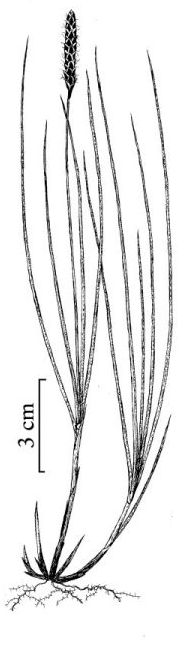
\includegraphics[scale=0.3]{images/carex.png}} \\
    & \\
    \textbf{Carex scirpoidea var. convoluta} & \\
    \textbf{Carex scirpoidea convoluta Kükenth.} & \\
    \textbf{Carex scirpoidea var. convoluta Kuk.} & \\
    \textbf{Carex scirpoidea var. convoluta Kük.} & \\
    \textbf{Carex scirpoidea var. convoluta Kükenth.} & \\
    \textbf{Carex scirpoidea var. convoluta Kükenthal} & \\
    \textbf{Carex scirpoidea Michx. var. convoluta Kük.} & \\
    \textbf{Carex scirpoidea Michx. var. convoluta Kükenth.} & \\
    \textbf{Carex scirpoidea Michaux var. convoluta Kükenthal} & \\
    & \\
    \textbf{Carex scirpoidea subsp. convoluta} & \\
    \textbf{Carex scirpoidea ssp. convoluta (Kük.) Dunlop} & \\
    \textbf{Carex scirpoidea subsp. convoluta (Kük.) Dunlop} & \\
    \textbf{Carex scirpoidea ssp. convoluta (Kukenth.) Dunlop} & \\
    \textbf{Carex scirpoidea subsp. convoluta (Kük.) D.A.Dunlop} & \\
    \textbf{Carex scirpoidea subsp. convoluta (Kük.) D.A. Dunlop} & \\
    \textbf{Carex scirpoidea Michx. ssp. convoluta (Kük.) Dunlop} & \\
    \textbf{Carex scirpoidea subsp. convoluta (Kuk.) D. A. Dunlop} & \\
    \textbf{Carex scirpoidea Michx. subsp. convoluta (Kük.) Dunlop} & \\
    \textbf{Carex scirpoidea Michx. ssp. convoluta (Kükenth.) Dunlop} & \\
    \textbf{Carex scirpoidea subsp. convoluta (Kükenthal) D.A. Dunlop} & \\
    \textbf{Carex scirpoidea Michx. subsp. convoluta (Kük.) D.A.Dunlop} & \\
    \textbf{Carex scirpoidea Michx. subsp. convoluta (Kük.) D.A. Dunlop} & \\
    \textbf{Carex scirpoidea subsp. convoluta (Kükenthal 1909) D.A. Dunlop 1998} & \\
    \hline
    \end{tabular}
  \end{center}
\end{table}

Table~\ref{table:carex} illustrates that there is no single correct way to
spell scientific names. As a result of the variations, exact string matching
links less than 15\% of entries in major data environments
\cite{Patterson:inpress-a}. In order to improve this metric, we need to
reconcile spelling variants with each other. The reconciliation process
involves linking alternative name-strings for the same taxon into
reconciliation groups. Most biologists will recognize the name-strings in Table
1 as referring to the same taxon, identifying elements (canonical form,
authors, ranks etc.) - that is ``parsing'' the name-strings.  This allows them
to mentally discard the less significant parts such as annotations and
authorship. It then becomes clear all of name-strings have a common ``canonical
form'' -- \textbf{Carex scirpoidea convoluta}. Further analysis of the
name-strings would reveal two different reconciliation groups:

\begin{itemize}

  \item \textbf{Carex scirpoidea var. convoluta} description by
    \textbf{Kükenthal}

  \item \textbf{Carex scirpoidea subsp. convoluta} rank change by
    \textbf{Dunlop}.

\end{itemize}

Initially such problem of normalizing scientific names by parsing had been
addressed as described above -- by manual means. A person familiar with
botanical rules of nomenclature would be able to analyse the example of 24
name-strings with relative ease, but not thousands and millions of
name-strings. The manual splitting of names into canonical form and the
authorship part is expensive, slow, inflexible and cannot elegantly deal with
name-strings where authorship is present in the middle of the name (for example
\textbf{Carex scirpoidea Michx. subsp.  convoluta (Kük.) D.A.Dunlop}).  This
requires an algorithmic solution, a scientific name parser!

An early algorithmic approach was to parse scientific names with regular
language implemented as regular expression \cite{Leary2007}. Regular expression
is a sequence of characters that describes a search pattern
\cite{aho1992foundations}. For example a regular expression ``[A-Z][a-z]\{2\}''
corresponds to a capitalized word from 3 letters like ``Zoo''. Examples of
parsers based on regular expressions are GBIF's \textit{name-parser}
\cite{gbifNameParser}, and \textit{YASMEEN} \cite{VandenBerghe2015}.

Regular expression is a powerful approach to string matching, but it has
limitations. For example regular expressions do not have facilities to deal
with recursive elements \cite{yu1997handbook} which may occur within scientific
names, such as hybrid formulae (for example \textbf{Brassica oleracea L.
subsp.  capitata (L.) DC. convar. fruticosa (Metzg.) Alef.  $\times$ B.
oleracea L. subsp. capitata (L.) var.  costata DC.}). Names parsing built on
regular expressions is impractical for complex name-strings.

Another limitation is that most regular expression software tools are ``black
boxes'' that allow limited interaction with the parsing process, and
information about the parsing context is limited. Developers cannot call a
procedure during a parsing event. As a result it is difficult to implement and
maintain such functionality as error recovery, detailed warnings, and
descriptions of errors.

We wanted an algorithm  able to deal with complex scientific names of broader
complexity to give more flexibility than a regular expression approach.  We
believe that a general use parser should satisfy the following requirements.

\begin{enumerate}

  \item \textbf{High Quality.} A parser should be able to break names into
    their semantic elements to the same standards that can be achieved by a
    trained nomenclaturalist or better. This will give confidence in the
    automated process and eliminate tedious and expensive manual work.

  \item \textbf{Global Scope.} A parser should be able to parse all types of
    scientific names, including the most complex name-strings such as hybrid
    formulae, multi-infraspecific names, names with multilevel authorships etc.
    No name-strings should be left unparsed, otherwise information attached to
    them may remain undiscoverable.

  \item \textbf{Parsing Completeness.} All information included into a
    name-string is important, not only the canonical form of the scientific
    name. Authorship, year, rank information allow us to distinguish homonyms,
    similar names, synonyms, spelling mistakes, or chresonyms from each other.
    This improves the performance of subsequent reconciliation.

  \item \textbf{Speed.} For large-scale aggregators, a parser needs to have a
    high throughput to collect data quickly, to serve users with minimum delay,
    and to reduce the costs of running the hardware used for parsing.

  \item \textbf{Accessibility.} To be available to the widest possible audience
    a parser should be released as a stand-alone program. It has to have a good
    documentation, be able to work as a library, to function as a command line
    tool, as a tool with graphical interface, and to run as a socket and
    RESTful services.

\end{enumerate}

These requirements became our design goals. Based on our experience with
prototype systems, we selected Parsing Expression Grammars and Scala language
for the following reasons.

\subsection*{Adoption of Parsing Expression Grammars}

Parsing Expression Grammars (PEG) \cite{Ford2004} is a recently introduced
method for parsing texts. PEG allows to define rules which describe a grammar
of a text. In our case such rules are used to deconstruct scientific names.
The rules are built from the ground up, staring from the simplest like
``character'' or ``space''. Then a ``genus'' rule would be a combination of a
``capital\_character'' followed by several ''lower\_case\_characters'',
``authorship'' would be a combination of several ``authors'' and optionally a
``year'', ``author'' would consist of ``author\_words'' etc. PEG rules are
designed to be recursive and easy to combine to new rules of ever increasing
complexity. Also each rule can have programmatic logic attached, making PEG
approach very introspective and flexible. We believe that PEG suites our goals
better than regular expressions for the following reasons:

\begin{itemize}

  \item PEG is better suited to texts with recursive syntax than, for example,
    regular expressions.

  \item scientific names' syntax is formal enough to be closer to an algebraic
    structure rather than to a natural language. Inconsistencies and
    ambiguities in scientific names are relatively rare due to adherence to
    nomenclatural codes.

  \item typically, scientific name-strings are short enough to avoid
    computational complexity and memory consumption

  \item programming a parser is easier than with regular expressions because
    PEG allows us to compose parsing rules in a clear domain specific language

  \item Such domain specific language offers great flexibility for logic within
    the rules, for example for reporting errors in name-strings.

\end{itemize}

In 2008, Global Names created a specialized parsing library
\textit{biodiversity} \cite{biodiversity} written in Ruby and based on PEG. We
used an excellent \textit{TreeTop} Ruby library \cite{treetop} as an underlying
PEG implementation.

The PEG approach allowed us to deal with complex scientific names gracefully.
It gave us flexibility to incorporate edge cases and to detect common mistakes
during the parsing process. The library \textit{biodiversity} enjoyed
considerable popularity. At the time of writing, it had been downloaded more
than 150,000 times \cite{bdiv-downloads}, it is used by many taxon name
resolution projects (e.g. Encyclopedia of Life \cite{eol}, Canadian Register of
Marine Species (CARMS) \cite{carms}, the iPlant TNRS \cite{iplant}, and World
Registry of Marine Species (WoRMS) \cite{worms}.  According to BioRuby
statistics \textit{biodiversity}, at the time of writing, had been the most
popular bio-library in Ruby language \cite{biogems}.

We were pleased with PEG approach for scientific names parsing, but now regard
the \textit{biodiversity} parser library as a working prototype that allowed us
to identify  problems and implement solutions for them.

\subsection*{Adoption of Scala}

The \textit{biodiversity} presented performance and scalability issues because
of the choice of Ruby as its programming language. Ruby is one of the best
languages for rapid prototyping, but it is an interpreted dynamic language with
originally a single-threaded runtime in a virtual machine. This makes it slow
and inappropriate for rapid service or large tasks. We determined that we
needed an environment with the following properties:

\begin{itemize}

    \item mature technology

    \item multi-threaded, with high performance and scalability

    \item active community with open-source friendly culture

    \item a wide range of libraries: utilities, web frameworks, etc.

    \item mature development environment: IDEs, testings frameworks, debuggers,
      profilers

    \item technologies for search and cluster computations

    \item interoperability with languages used in scientific community (R,
      Python, Matlab)

    \item natural support of domain specific languages embedded in hosted
      language

\end{itemize}

While many of the properties are true for Ruby, but others, such as high
performance, scalability and interoperability are lacking. To meet all
requirements, and exploiting what we had learned from \textit{biodiversity}, we
refactored it to fulfil all requirements using Java virtual machine, Scala
programming language \cite{odersky2004overview}, and the Open Source
\textit{Parboiled2} library \cite{parboiled2} which implements PEG in Scala. An
alternative to \textit{parboiled2} is the Scala parser combinators library
\cite{moors2008parser} but has known problems with speed and memory consumption
making \textit{parboiled2} our preferred choice.

The functional programming features of Scala allowed us to build a custom
parsing language that describes the rules of the grammars of scientific names.
This produces Parsing Expression Grammar that provides considerably more
flexibility than external Lexers such as Bison or Yacc. As this domain specific
language is within \textit{Parboiled2} it can take advantage of the Macro
capacity of Scala \cite{Burmako:2013:SML:2489837.2489840} to modify the
compiler and how the program operates. The result is that the software operates
with high efficiency.

With this combination, the resulting \textit{gnparser} achieved a significant
boost in speed, scalability, and portability of the library.  We limited this
version to work with scientific names that complied with the botanical,
zoological, and prokaryotic codes, but not with names of viruses which are
formed in different ways \cite{ICTV, Patterson:inpress-a}

\section*{Implementation}

The \textit{gnparser} project is entirely written in Scala. It supports two
major Scala versions: 2.10.3+ and 2.11.x. The code is organized into four
modules (or subprojects in Scala terminology).

TODO: FIGURE OF AN ABSTRACT SYNTAX TREE EXAMPLE FOR A NAME-STRING

\begin{enumerate}

  \item ``\textit{parser}'' is the core module used by all other modules. It
    contains the components for successful parsing of scientific names: parsing
    grammar, abstract syntax tree (AST) composed of a scientific name
    components (refer to Table), warnings and error facilities.  When the
    parsing is complete and elements of name-strings have been assigned to the
    syntax tree, then the elments can be formatted to meet further needs.  For
    example:

\begin{itemize}

  \item \textit{normalizer} is to convert input name-strings into a consistent
    style;

  \item \textit{canonizer} to create canonical forms of the names; and

  \item \textit{JSON renderer}  $Result$ is converted to JSON
    \cite{bray2014javascript} to allow developers familiar with other languages
    to work with the output.  The output has the following information:


\textbf{details} contains the JSON-representation of a parsed scientific name

\textbf{quality\_warnings} describes potential problems if names are not
well-formed

\textbf{quality} depicts a quality level of the parsed name

\textbf{positions} maps the positions of every element in a parsed name to the
semantic meaning of the element

Full and formal explanation of all parser's fields is given as a JSON schema
can be found online \cite{gnparser-json}.

\end{itemize}

  \item ``\textit{examples}'' contains  examples to assist developers in
    building \textit{parser} into other popular programming languages: Java,
    Scala, Python, Ruby, and R

  \item ``\textit{runner}'' contains the code that allows users to run
    ``\textit{parser}'' from a command line as a standalone tool or to run it
    as a TCP/IP socket server. ``\textit{runner}'' depends on the
    ``\textit{parser}''.   The core part is the launch script
    ``\textit{gnparse}'' (for Linux/Mac and Windows) that creates JVM instance
    and runs ``\textit{parser}'' on multiple threads against the input provided
    via a socket or file.

  \item ``\textit{web}'' contains a web application and a RESTful interface as
    a simpler method to access ``\textit{parser}''. It is a Play Framework
    \cite{wampler2011scala} application. It depends on the ``\textit{parser}''
    library. ``\textit{web}'' achieves interactions with ``\textit{parser}''
    via HTTP protocols. It works both with simple HTML and REST API interfaces
    Figure~\ref{figure:webgui} shows a parsing example using the web-interface.

\end{enumerate}

All subprojects but ``\textit{web}'' can run in JVM 1.6. ``\textit{web}''
requires JVM 1.8.

\begin{figure}[htbp]
  \begin{center}

    \caption{Web Graphical User Interface \cite{gnparser-web}. In this example
      a user entered a name-string of a hybrid name consisted of 21 elements.
      The ``Results'' section contains detailed parsed output using compact
      JSON format.}\label{figure:webgui}

    \vspace{5mm}
    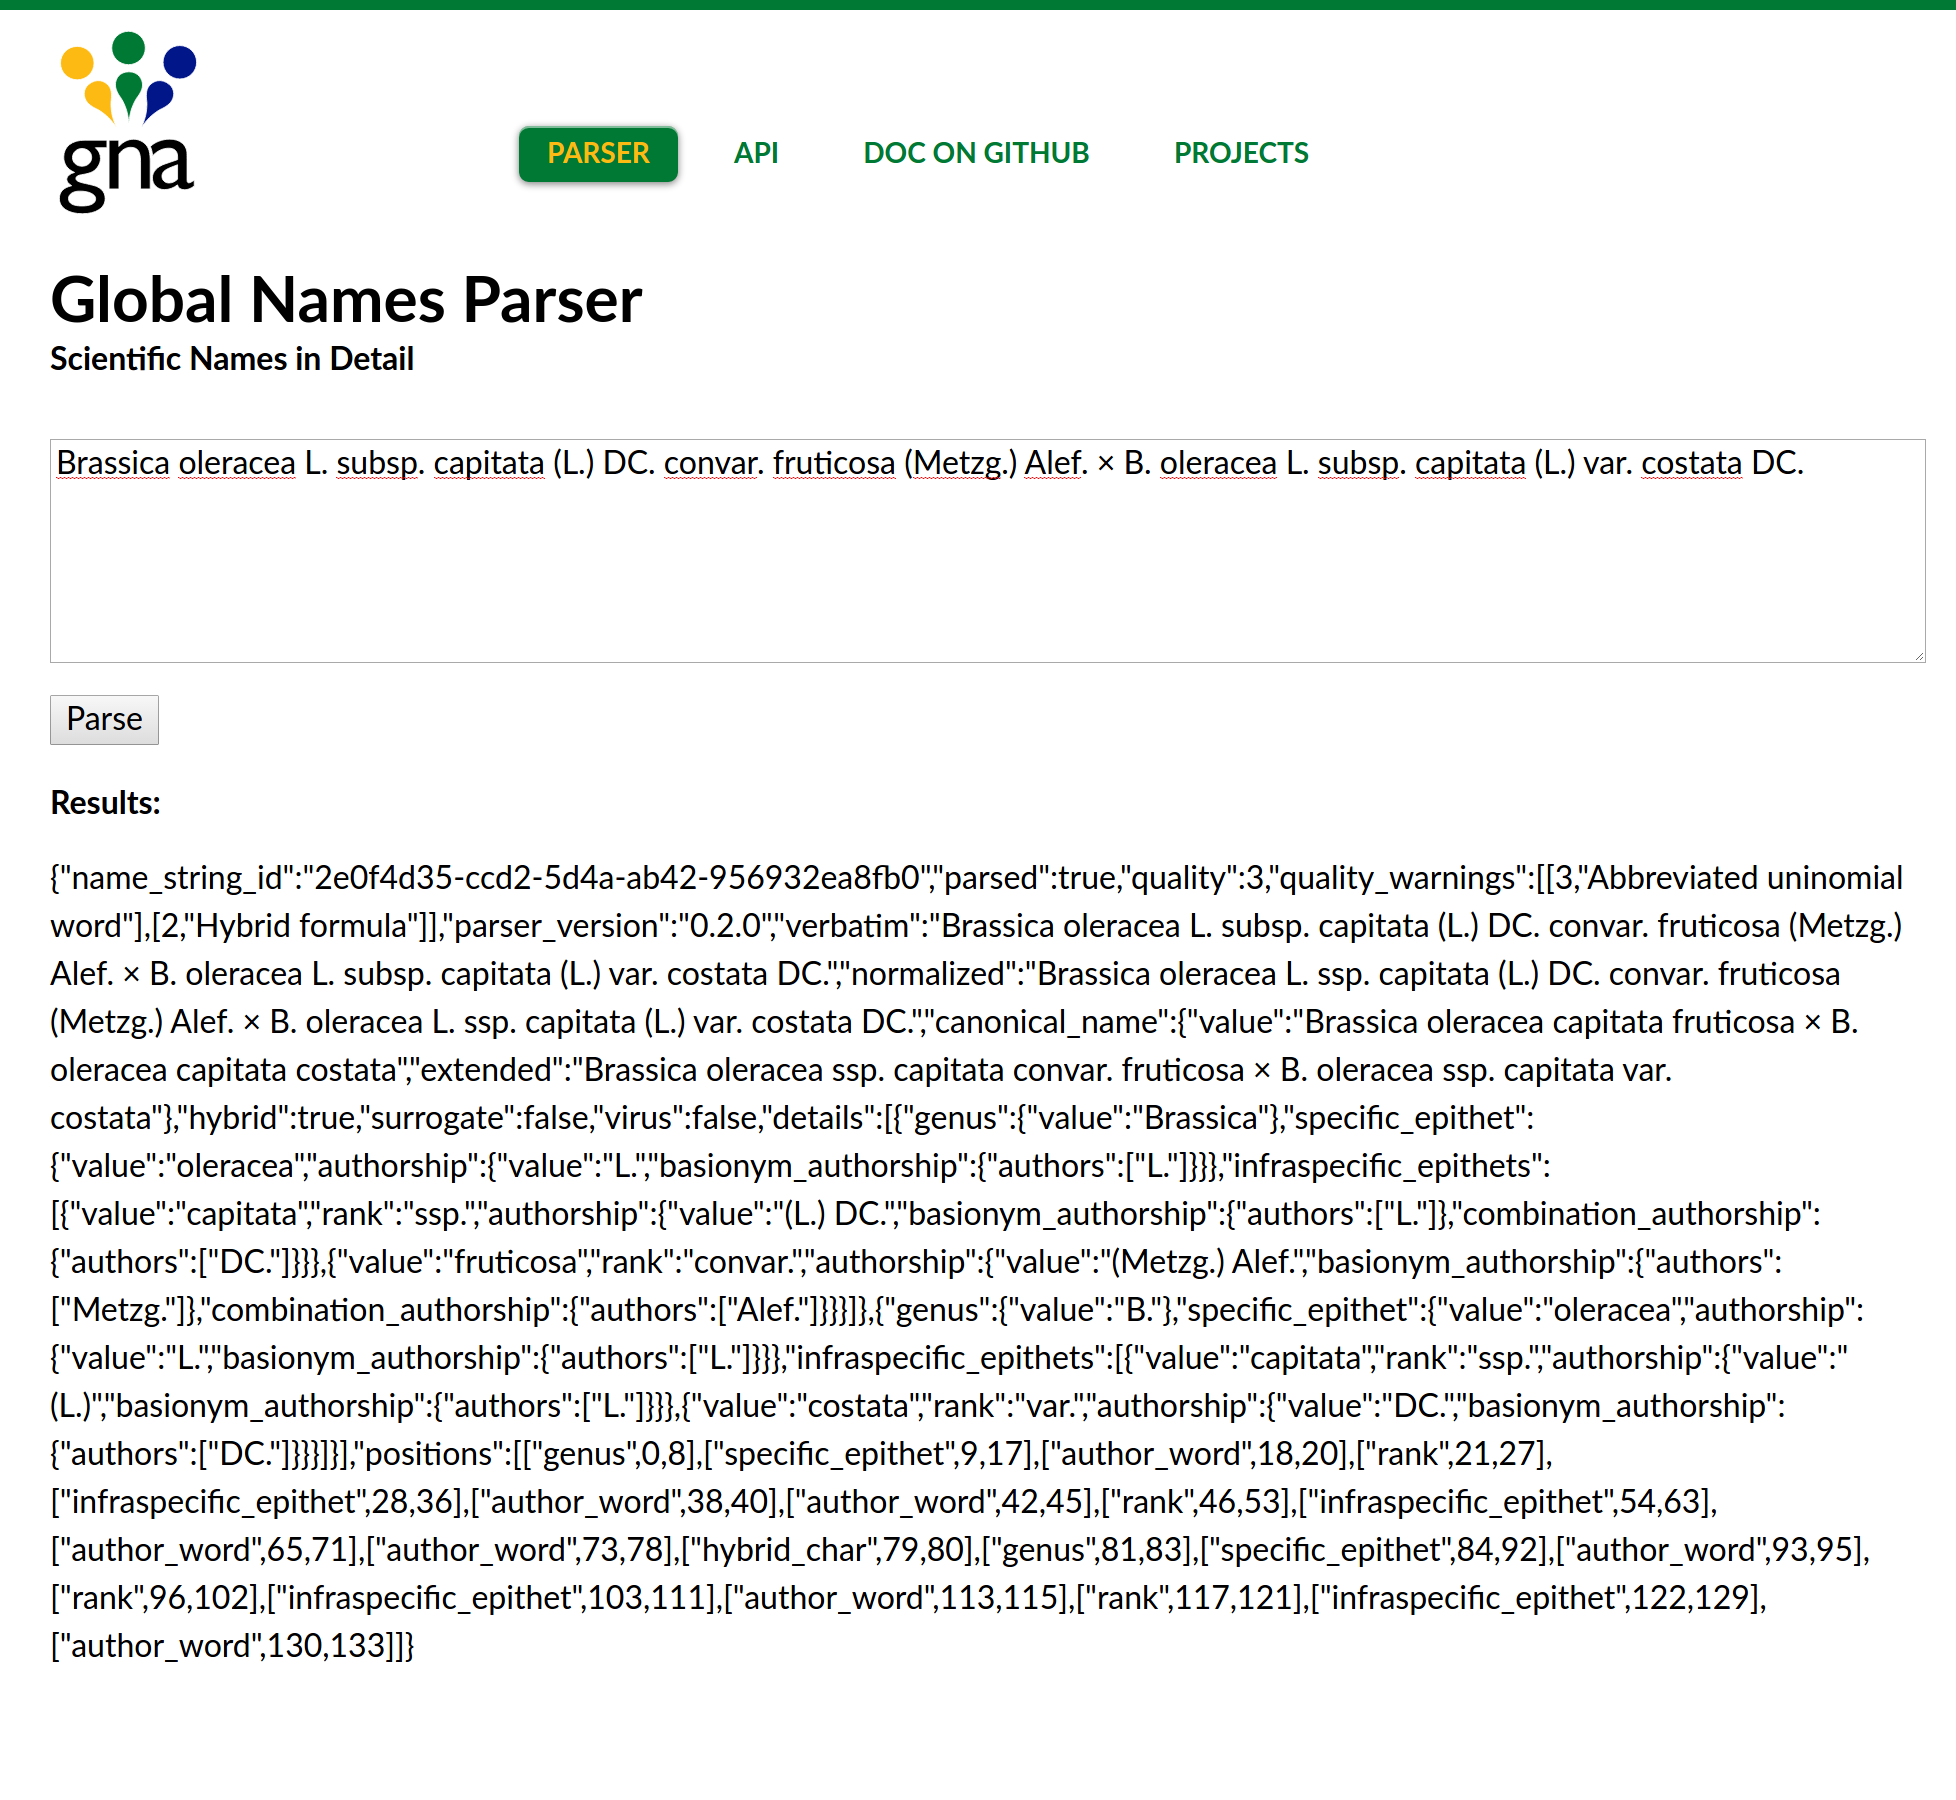
\includegraphics[scale=0.175]{images/web_gui.png}
  \end{center}
\end{figure}

Documentation is available in a README file (see section ``Availability and
Requirements).

\subsection*{Installation}

``\textit{gnparser}'' is available for launch in three bundles:

\begin{itemize}

  \item A \textit{parser} artifact is provided via Maven central repository of
    Java code (REF!). Physically it is a relatively small jar file without
    external dependencies. The artifact can be accessed by a build system such
    as Maven, Gradle, or SBT in other projects. The build system then
    identifies and provides access to any other required code-dependencies.

  \item A Zip-archived ``fat jar'' is located at the project's GitHub
    repository.  The jar contains the compiled files of \textit{gnparser} along
    with all necessary dependencies to launch it within JVM. The archive is
    also bundled with a launch script (for Windows, OS X and Linux) that can
    run a command line interface to \textit{gnparser}.

  \item The project's Docker container is located at Docker hub  (*REF!).
    Docker provides an additional layer of abstraction and automation of
    operating-system-level virtualization on Linux. It can be thought as
    lightweight virtualization technology within same Linux OS process. When it
    is setup properly, everything -- starting from JVM and ending with Scala
    and SBT -- can be run with simple commands that will, for example,  pull
    the Docker image from the Hub, and run the socket or web server on a
    desired port.

\end{itemize}

\subsection*{Testing Methods}

Data for our tests (1,000 and 100,000 name-strings) were randomly chosen from
24 million name-strings of the Global Names Index \cite{gn:index}. These
resulting datasets consisted of strings acquired from a variety of data sources
and were a mixture of well-formed names, names with formatting and spelling
mistakes, and name-strings that were misrepresented as names.

We compared performance of \textit{gnparser} with 2 other projects --
\textit{biodiversity} parser \cite{Boyle2013, biodiversity} (also developed by
Global Names), and GBIF \textit{name-parser} \cite{gbifNameParser}. For
comparisons we calculated $Precision$, $Recall$ and $Accuracy$ (as described
below) using a dataset consisted of 1000 name-strings. Another project we
considered was YASMEEN parser from iMarine project \cite{VandenBerghe2015},
however we found that with our dataset it generated dramatically more mistakes
than other parsers ($Precision$ 0.534, $Recall$ 1.0, $F1$ 0.6962), and was
unable to finish full dataset without crashing. We excluded it from further
tests.

To estimate the quality for the parsers we needed a feature that is common to
all three of them and is a good indicator of performance.  We decided to use a
combination of canonical form and terminal authorship.  The canonical form
represents the essential elements of a name, while the terminal authorship
refers to the authority of the lowest subtaxon  referred to in the name. For
example in \textbf{Oriastrum lycopodioides Wedd.  var.  glabriusculum Reiche}
canonical form is \textbf{Oriastrum lycopodioides glabriusculum} and terminal
authorship is \textbf{Reiche}, not \textbf{Wedd.}.

When both the canonical form and the terminal authorship were determined
correctly we marked the result as true positive ($\text{tp}$).  If one or both
of them were determined incorrectly, the result was marked a false positive
($\text{fp}$). Name-strings correctly discarded from parsing were marked as
true negatives ($\text{tn}$). False negatives ($\text{fn}$) were ``suitable''
name-strings which should be parsed, but were not The
following parameters where used for analysis:

$Accuracy$ -- a proportion of correct results to all results.  It is calculated
as:

\[Accuracy = \dfrac{\text{tp} + \text{tn}} {\text{tp} + \text{tn} + \text{fp} +
    \text{fn}}\]

$Precision$ -- a proportion of name-strings parsed correctly to all detected
name-strings. It is is calculated as:

\[Precision = \dfrac{\text{tp}}{(\text{tp} + \text{fp})}\]

$Recall$ -- a proportion of correctly detected name-strings to all parseable
name-strings and calculated as:

\[Recall = \dfrac{\text{tp}}{(\text{tp} + \text{fn})}\]

$F1-measure$ is a balanced harmonic mean (where $Precision$ and $Recall$ have
the same weight). When both $Precision$ and $Recall$ vary, $F1-measure$ allows
results to be compared. It is calculated as

\[F1 = \dfrac{2 \times Precision \times Recall}{(Precision + Recall)}\]

Parsers can analyze the structure of name-strings, but they cannot determine if
a string is a ``real'' name. For example, in the case of a name-string that has
the same form as a subspecies such as \textbf{"Example name Word var. something
Capitalized Words, 1900"}. In such a case, the identification of a canonical
form as \textbf{"Example name something"} and terminal authorship as
\textbf{"Capitalized Words, 1900"} would be considered a true positive.

Some names in the dataset were not well-formed. If a human could extract the
canonical form and the terminal authorship from them, we included them.
Examples of such name-strings are \textbf{"Bumetopia (bumetopia) quadripunctata
Breuning"} (lower case initial letter of the subgenus), \textbf{"Campylium
gollanii C. M?ller ex Vohra 1970 [1972]"} (a miscoded UTF-8 symbol and an
additional year in square brackets), \textbf{"Myosorex muricauda (Miller,
1900)."} (with a period after the authorship).

It is important for a parser to accurately distinguish between name-strings of
scientific names, names of viruses, surrogate names, and non-names. To find out
how well parsers distinguished strings which are not scientific names, we
calculated $Precision$ for discarded/non-parsed strings. If done correctly
not-parsed strings would include only names of viruses and terms that do not
comply with the zoological, prokaryotic, and botanical Codes of nomenclature.

We processed 100,000 name-strings with each parser.  Each parser discarded
close to 1000 name-strings as not-parseable.  $Precision$ in this case showed
percentage of correctly discarded names.  We do not know $Recall$, as it was
not reasonable to manually determine this for 100,000 names. To get a sense of
names which had to be discarded, but were parsed instead, we analysed
intersections and differences of the results between the three parsers.

To establish the throughput of parsing we used a computer with an Intel
i7-4930K CPU (6 cores, 12 threads, at 3.4 GHz), 64GB of memory, and 250GB
Samsung 840 EVO SSD, running Ubuntu version 14.04. Throughput was determined by
processing of 1,000,000 random name-strings from GNI.

To study effects of parallel execution on throughput we used the
\textit{ParallelParser} class from \textit{biodiversity} parser and
\textit{gnparse} a command line interface for \textit{gnparser}. For GBIF
\textit{name-parser}, we created a thin wrapper with multi-threaded
capabilities \cite{gbifparser}.

\section*{Results and Discussion}

We discuss \textit{gnparser}, GBIF \textit{name-parser} and
\textit{biodiversity} parser from the point of the 5 requirements mentioned
above.

\begin{enumerate}
  \item High Quality Parsing
  \item Global Scope
  \item Parsing Completeness
  \item Speed
  \item Accessibility
\end{enumerate}

\subsection*{High Quality Parsing}

High quality parsing is the most important out of the 5 requirements.  We
compared \textit{gnparser} together with 2 other approaches to parsing that
represent state of the art for parsing biological scientific names. GBIF
\textit{name-parser} uses regular expressions approach, while \textit{gnparser}
and \textit{biodiversity} parsers use PEG approach.  Results for our quality
measurements are shown in Table~\ref{table:precision}.

If the test data contain a large proportion of true negatives ($\text{tn}$)
$Accuracy$ is not a good measure as it favors algorithms which distinguish
negative results, rather than finding positive ones. By manual checking, we
established that our test datasets had only $\approx1\%$ of non-scientific
names. As true negatives were rare, they had very little influence on results.
$Recall$ for all parsers was very high, which means false negatives had an
insignificant influence on results. We hold that $Accuracy$ is the best measure
for our tests and is sufficient to compare quality for all cases.

Altogether we find that all 3 parsers performed very well with $Accuracy$
values higher than $95\%$. Both \textit{gnparser} and \textit{biodiversity}
parser approached 99\% mark which we regard as production quality. Moreover,
most of the false positives came from name-strings with mistakes. For example
Out of 11 false positives (below) that \textit{gnparser} found in the 1000
name-string test data set, only 2 (the first 2) were well-formed names:

\vspace{0.5cm}

\begin{verbatim}
    Eucalyptus subser. Regulares Brooker
    Jacquemontia spiciflora (Choisy) Hall. fil.

    Acanthocephala declivis variety guianensis Osborn, 1904
    Atysa (?) frontalis
    Bumetopia (bumetopia) quadripunctata Breuning, 1950
    Cyclotella kã¼tzingiana Thwaites
    Elaphidion (romaleum) tæniatum Leconte, 1873
    Hieracium nobile subsp. perclusum (Arv. -Touv. ) O. Bolòs & Vigo
    Leptomitus vitreus (Roth) Agardh{?}
    Myosorex muricauda (Miller, 1900).
    Papillaria amblyacis (M<81>ll.Hal.) A.Jaeger
\end{verbatim}

\vspace{0.5cm}

As illustrated by these examples, we expect parsers to deal with mistakes,
annotations, and Unicode characters miscodings. To alert users,
\textit{gnparser} generates warnings for each problem it identified in a
name-string. The other parsers do not have this feature.

When parsers reach $\approx80\%$ $Accuracy$, they hit a ``long tail'' of
problems where each particular type of a problem is rare, yet every new manual
test against 1,000-10,000 name-strings reveals new issues.  Examples of these
challenges are given elsewhere \cite{Patterson:inpress-a}. For all three
parsers, developers performed the meticulous task of adding one rare case after
another to the list of problems and finding ways to incorporate solutions. That
is, parsers need to be subject to continuous improvement. The problems found
during preparation of this paper are being addressed in the next version of
\textit{gnparser} as well. As the parsing rules improve, we believe that
\textit{gnparser} can reach $>99.5\%$ $Accuracy$ without diminishing $Recall$.

As we incorporate new rules to increase $Recall$, we have to consider the risks
of reducing $Precision$ by introducing new false positives. For example GBIF
\textit{name-parser} allows the genus element of a name-string to start with a
lowercase character. As a result the name-strings below were parsed as if they
were scientific names, while other parsers ignored them:

\vspace{0.5cm}

\begin{verbatim}
    acid mine drainage metagenome
    agricultural soil bacterium CRS5639T18-1
    agricultural soil bacterium SC-I-8
    algal symbiont of Cladonia variegata MN075
    alpha proteobacterium AP-24
    anaerobic bacterium ANA No.5
    anoxygenic photosynthetic bacterium G16
    archaeon enrichment culture clone AOM-SR-A23
    bacterium endosymbiont of Plateumaris fulvipes
    bacterium enrichment culture DGGE band 61_3_FG_L
    barley rhizosphere bacterium JJ-220
    bovine rumen bacterium niuO17
\end{verbatim}

\vspace{0.5cm}

Solutions like these might increase $Recall$ with certain low-quality datasets,
but they also may decrease $Precision$ with other datasets. When dealing with
``dirty'' datasets containing predictable problems, we find the best solution
is to include a ``preparser'' script which ``normalizes'' known problems  and
then apply a high quality parser to the result.  As an example, DRYAD contained
many name-strings in which elements of scientific names had been concatenated
with an interpolated character such as `\_’ (e.g. ``Homo\_sapiens'' and
``Pinoyscincus\_jagori\_grandis'') \cite{Patterson:inpress-a}.

Our testing also revealed differences between regular expressions and PEG
approaches. Both can achieve high quality results with canonical forms, but the
regular expressions approach is less suitable for more complex name-strings.
The reason for this is the recursive nature of scientific names.  It is
relatively straightforward to parse ``simple'' name-strings with regular
expressions, but the recursive nature of some names-strings present greater
problems that at some point become unsurmountable.

\subsection*{Global Scope}

If we want to connect biological data using scientific names, no name-strings
should be missed or rejected, no matter how complex they are. During our
testing we found that $Accuracy$ of GBIF \textit{name-parser} was negatively
affected by not dealing with hybrid formulae and infrasubspecific names (names
with more then one infraspecific epithet). Regular expressions do not support
recursion meaning that more complex names are harder to parse.  For example the
following names were not supported by GBIF \textit{name-parser}:

\vspace{0.5cm}

\begin{verbatim}
    Crataegus chlorosarca subtaxon pubescens E.L.Wolf
    Erigeron peregrinus ssp.callianthemus var. eucallianthemus
    Salvelinus fontinalis x Salmo gairdneri
    Echinocereus fasciculatus var. bonkerae × E. fasciculatus
      var. fasciculatus
\end{verbatim}

\vspace{0.5cm}

We use PEG approach because it supports nesting parsing rules within each other,
and creates progressively more and more complex rules. The first rule defines a
space between words, the last rule defines hybrid formulas.  Such support for
recursion allows \textit{gnparser} to handle full spectrum of scientific names.

\begin{table}[htb]
  \begin{center}
    \caption{Precision/Recall for processed by parsers 1000
    name-strings}\label{table:precision}
    \resizebox{10cm}{!} {
    \begin{tabular}{|l|*{3}{l}|}
      \hline
                             & gnparser & gbif-parser & biodiversity \\
      \hline
      \textit{True Positive} & 976      & 955         & 971          \\
      \textit{True Negative} & 13       & 12          & 13           \\
      \textit{False Positive}& 11       & 32          & 16           \\
      \textit{False Negative}& 0        & 1           & 0            \\
      \textit{Precision}     & 0.9888551& 0.967578    & 0.9837893    \\
      \textit{Recall}        & 1.0      & 0.998954    & 1.0          \\
      \textit{F1}            & 0.9943963& 0.983016    & 0.9918284    \\
      \textit{Accuracy}      & 0.989    & 0.967       & 0.984        \\
      \hline
    \end{tabular}
    }
  \end{center}
\end{table}

\begin{table}[htb]
  \begin{center}
    \caption{Precision for discarded by parsers names, out of 100 000
    name-strings}\label{table:unparsed}
    \resizebox{10cm}{!} {
    \begin{tabular}{| l | *{3}{l} |}
      \hline
                              & gnparser & gbif-parser & biodiversity \\
      \hline
      \textit{Total discarded}& 1131     & 1082        & 1161         \\
      \textit{True Positive}  & 1129     & 940         & 1152         \\
      \textit{False Positive} & 2        & 142         & 9            \\
      \textit{Precision}      & 0.998231 & 0.868761    & 0.9922481    \\
      \hline
    \end{tabular}
  }
  \end{center}
\end{table}

\begin{figure}[htbp]
  \begin{center}
    \caption{
      Names parsed per second by GN, GBIF and Biodiversity parsers
      (running on 1-12 parallel threads).
    }\label{figure:throughput}
    \vspace{0.5cm}
    \begin{tabular}{| l | *{3}{r} | c c c |}
      \hline
      \multirow{1}{*}Threads & gnparser & gbif-paser & biodiversity
      & \multicolumn{3}{c |}{Ratio} \\
      \cline{5-7}
      & & & & gn & gbif & bio \\
      \hline
      1  & 5944  & 6389  & 1111 & 1 & 1.07 & 0.19 \\
      2  & 11416 & 12638 & 1722 & 1 & 1.11 & 0.14 \\
      4  & 20500 & 21994 & 2556 & 1 & 1.07 & 0.12 \\
      8  & 24805 & 30972 & 2777 & 1 & 1.25 & 0.11 \\
      12 & 26055 & 31833 & 2527 & 1 & 1.22 & 0.10 \\
      \hline
    \end{tabular}
    % Created by tikzDevice version 0.9 on 2015-12-21 16:35:00
% !TEX encoding = UTF-8 Unicode
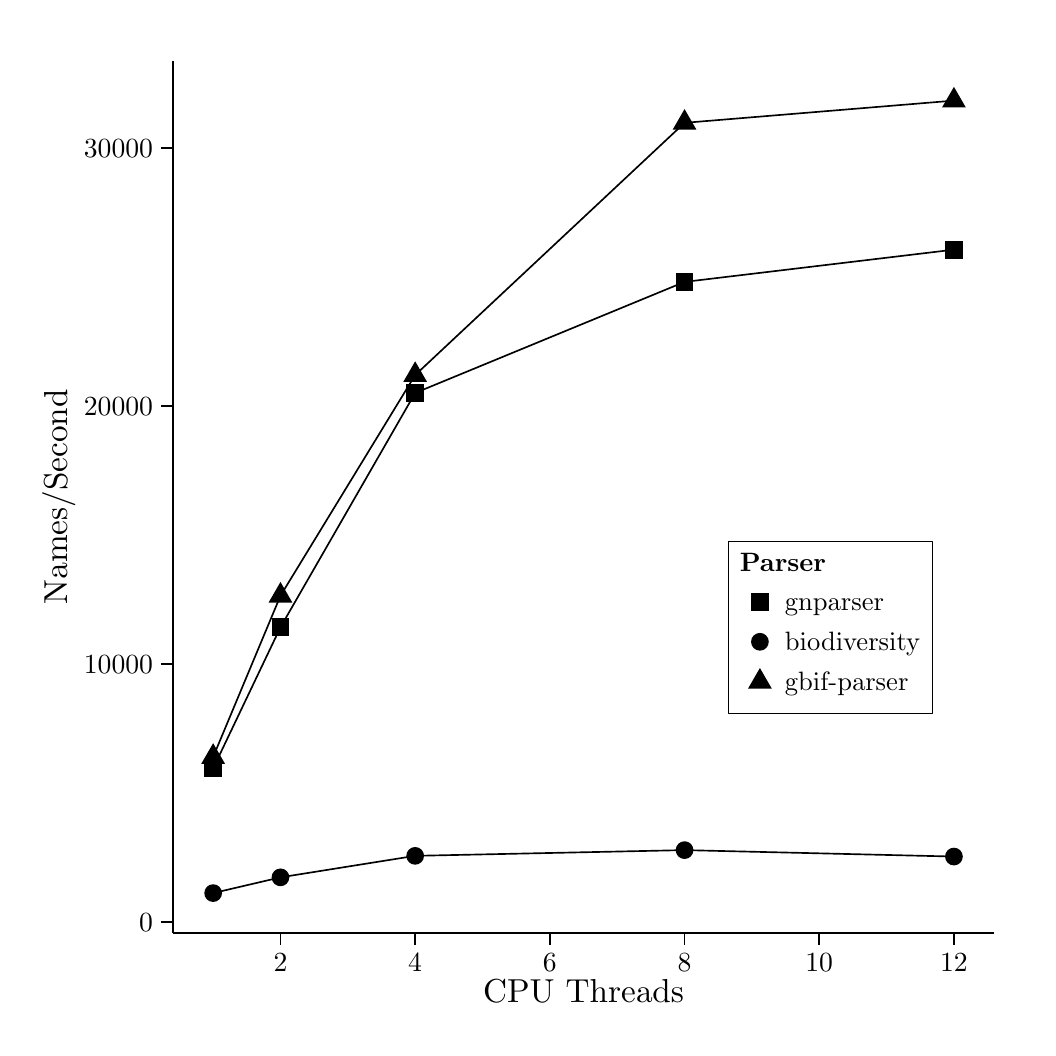
\begin{tikzpicture}[x=1pt,y=1pt]
\definecolor{fillColor}{RGB}{255,255,255}
\path[use as bounding box,fill=fillColor,fill opacity=0.00] (0,0) rectangle (361.35,361.35);
\begin{scope}
\path[clip] (  0.00,  0.00) rectangle (361.35,361.35);
\definecolor{drawColor}{RGB}{255,255,255}
\definecolor{fillColor}{RGB}{255,255,255}

\path[draw=drawColor,line width= 0.6pt,line join=round,line cap=round,fill=fillColor] (  0.00,  0.00) rectangle (361.35,361.35);
\end{scope}
\begin{scope}
\path[clip] ( 52.42, 34.31) rectangle (349.30,349.30);
\definecolor{fillColor}{RGB}{255,255,255}

\path[fill=fillColor] ( 52.42, 34.31) rectangle (349.30,349.30);
\definecolor{drawColor}{RGB}{255,255,255}

\path[draw=drawColor,line width= 0.6pt,line join=round] ( 52.42, 38.27) --
	(349.30, 38.27);

\path[draw=drawColor,line width= 0.6pt,line join=round] ( 52.42,131.48) --
	(349.30,131.48);

\path[draw=drawColor,line width= 0.6pt,line join=round] ( 52.42,224.69) --
	(349.30,224.69);

\path[draw=drawColor,line width= 0.6pt,line join=round] ( 52.42,317.90) --
	(349.30,317.90);

\path[draw=drawColor,line width= 0.6pt,line join=round] ( 91.35, 34.31) --
	( 91.35,349.30);

\path[draw=drawColor,line width= 0.6pt,line join=round] (140.02, 34.31) --
	(140.02,349.30);

\path[draw=drawColor,line width= 0.6pt,line join=round] (188.69, 34.31) --
	(188.69,349.30);

\path[draw=drawColor,line width= 0.6pt,line join=round] (237.36, 34.31) --
	(237.36,349.30);

\path[draw=drawColor,line width= 0.6pt,line join=round] (286.03, 34.31) --
	(286.03,349.30);

\path[draw=drawColor,line width= 0.6pt,line join=round] (334.70, 34.31) --
	(334.70,349.30);
\definecolor{drawColor}{RGB}{0,0,0}

\path[draw=drawColor,line width= 0.6pt,line join=round] ( 67.02, 48.63) --
	( 91.35, 54.32) --
	(140.02, 62.09) --
	(237.36, 64.16) --
	(334.70, 61.83);

\path[draw=drawColor,line width= 0.6pt,line join=round] ( 67.02, 97.82) --
	( 91.35,156.08) --
	(140.02,235.82) --
	(237.36,326.96) --
	(334.70,334.99);

\path[draw=drawColor,line width= 0.6pt,line join=round] ( 67.02, 93.68) --
	( 91.35,144.69) --
	(140.02,229.35) --
	(237.36,269.48) --
	(334.70,281.13);
\definecolor{fillColor}{RGB}{0,0,0}

\path[fill=fillColor] ( 63.82, 90.48) --
	( 70.22, 90.48) --
	( 70.22, 96.88) --
	( 63.82, 96.88) --
	cycle;

\path[fill=fillColor] ( 88.15,141.48) --
	( 94.55,141.48) --
	( 94.55,147.89) --
	( 88.15,147.89) --
	cycle;

\path[fill=fillColor] (136.82,226.15) --
	(143.22,226.15) --
	(143.22,232.55) --
	(136.82,232.55) --
	cycle;

\path[fill=fillColor] (234.16,266.28) --
	(240.56,266.28) --
	(240.56,272.68) --
	(234.16,272.68) --
	cycle;

\path[fill=fillColor] (331.50,277.93) --
	(337.90,277.93) --
	(337.90,284.33) --
	(331.50,284.33) --
	cycle;

\path[fill=fillColor] ( 67.02,102.80) --
	( 71.33, 95.33) --
	( 62.71, 95.33) --
	cycle;

\path[fill=fillColor] ( 91.35,161.06) --
	( 95.66,153.59) --
	( 87.04,153.59) --
	cycle;

\path[fill=fillColor] (140.02,240.80) --
	(144.33,233.33) --
	(135.71,233.33) --
	cycle;

\path[fill=fillColor] (237.36,331.94) --
	(241.67,324.47) --
	(233.05,324.47) --
	cycle;

\path[fill=fillColor] (334.70,339.96) --
	(339.01,332.50) --
	(330.39,332.50) --
	cycle;

\path[fill=fillColor] ( 67.02, 48.63) circle (  3.20);

\path[fill=fillColor] ( 91.35, 54.32) circle (  3.20);

\path[fill=fillColor] (140.02, 62.09) circle (  3.20);

\path[fill=fillColor] (237.36, 64.16) circle (  3.20);

\path[fill=fillColor] (334.70, 61.83) circle (  3.20);
\end{scope}
\begin{scope}
\path[clip] (  0.00,  0.00) rectangle (361.35,361.35);
\definecolor{drawColor}{RGB}{0,0,0}

\path[draw=drawColor,line width= 0.6pt,line join=round] ( 52.42, 34.31) --
	( 52.42,349.30);
\end{scope}
\begin{scope}
\path[clip] (  0.00,  0.00) rectangle (361.35,361.35);
\definecolor{drawColor}{RGB}{0,0,0}

\node[text=drawColor,anchor=base east,inner sep=0pt, outer sep=0pt, scale=  1.00] at ( 45.30, 34.83) {0};

\node[text=drawColor,anchor=base east,inner sep=0pt, outer sep=0pt, scale=  1.00] at ( 45.30,128.04) {10000};

\node[text=drawColor,anchor=base east,inner sep=0pt, outer sep=0pt, scale=  1.00] at ( 45.30,221.25) {20000};

\node[text=drawColor,anchor=base east,inner sep=0pt, outer sep=0pt, scale=  1.00] at ( 45.30,314.46) {30000};
\end{scope}
\begin{scope}
\path[clip] (  0.00,  0.00) rectangle (361.35,361.35);
\definecolor{drawColor}{RGB}{0,0,0}

\path[draw=drawColor,line width= 0.6pt,line join=round] ( 48.15, 38.27) --
	( 52.42, 38.27);

\path[draw=drawColor,line width= 0.6pt,line join=round] ( 48.15,131.48) --
	( 52.42,131.48);

\path[draw=drawColor,line width= 0.6pt,line join=round] ( 48.15,224.69) --
	( 52.42,224.69);

\path[draw=drawColor,line width= 0.6pt,line join=round] ( 48.15,317.90) --
	( 52.42,317.90);
\end{scope}
\begin{scope}
\path[clip] (  0.00,  0.00) rectangle (361.35,361.35);
\definecolor{drawColor}{RGB}{0,0,0}

\path[draw=drawColor,line width= 0.6pt,line join=round] ( 52.42, 34.31) --
	(349.30, 34.31);
\end{scope}
\begin{scope}
\path[clip] (  0.00,  0.00) rectangle (361.35,361.35);
\definecolor{drawColor}{RGB}{0,0,0}

\path[draw=drawColor,line width= 0.6pt,line join=round] ( 91.35, 30.04) --
	( 91.35, 34.31);

\path[draw=drawColor,line width= 0.6pt,line join=round] (140.02, 30.04) --
	(140.02, 34.31);

\path[draw=drawColor,line width= 0.6pt,line join=round] (188.69, 30.04) --
	(188.69, 34.31);

\path[draw=drawColor,line width= 0.6pt,line join=round] (237.36, 30.04) --
	(237.36, 34.31);

\path[draw=drawColor,line width= 0.6pt,line join=round] (286.03, 30.04) --
	(286.03, 34.31);

\path[draw=drawColor,line width= 0.6pt,line join=round] (334.70, 30.04) --
	(334.70, 34.31);
\end{scope}
\begin{scope}
\path[clip] (  0.00,  0.00) rectangle (361.35,361.35);
\definecolor{drawColor}{RGB}{0,0,0}

\node[text=drawColor,anchor=base,inner sep=0pt, outer sep=0pt, scale=  1.00] at ( 91.35, 20.31) {2};

\node[text=drawColor,anchor=base,inner sep=0pt, outer sep=0pt, scale=  1.00] at (140.02, 20.31) {4};

\node[text=drawColor,anchor=base,inner sep=0pt, outer sep=0pt, scale=  1.00] at (188.69, 20.31) {6};

\node[text=drawColor,anchor=base,inner sep=0pt, outer sep=0pt, scale=  1.00] at (237.36, 20.31) {8};

\node[text=drawColor,anchor=base,inner sep=0pt, outer sep=0pt, scale=  1.00] at (286.03, 20.31) {10};

\node[text=drawColor,anchor=base,inner sep=0pt, outer sep=0pt, scale=  1.00] at (334.70, 20.31) {12};
\end{scope}
\begin{scope}
\path[clip] (  0.00,  0.00) rectangle (361.35,361.35);
\definecolor{drawColor}{RGB}{0,0,0}

\node[text=drawColor,anchor=base,inner sep=0pt, outer sep=0pt, scale=  1.20] at (200.86,  9.03) {CPU Threads};
\end{scope}
\begin{scope}
\path[clip] (  0.00,  0.00) rectangle (361.35,361.35);
\definecolor{drawColor}{RGB}{0,0,0}

\node[text=drawColor,rotate= 90.00,anchor=base,inner sep=0pt, outer sep=0pt, scale=  1.20] at ( 14.29,191.81) {Names/Second};
\end{scope}
\begin{scope}
\path[clip] (  0.00,  0.00) rectangle (361.35,361.35);
\definecolor{drawColor}{RGB}{0,0,0}
\definecolor{fillColor}{RGB}{255,255,255}

\path[draw=drawColor,line width= 0.3pt,line join=round,line cap=round,fill=fillColor] (253.09,113.49) rectangle (326.76,175.63);
\end{scope}
\begin{scope}
\path[clip] (  0.00,  0.00) rectangle (361.35,361.35);
\definecolor{drawColor}{RGB}{0,0,0}

\node[text=drawColor,anchor=base west,inner sep=0pt, outer sep=0pt, scale=  0.96] at (257.36,164.73) {\bfseries Parser};
\end{scope}
\begin{scope}
\path[clip] (  0.00,  0.00) rectangle (361.35,361.35);
\definecolor{drawColor}{RGB}{255,255,255}
\definecolor{fillColor}{RGB}{255,255,255}

\path[draw=drawColor,line width= 0.6pt,line join=round,line cap=round,fill=fillColor] (257.36,146.67) rectangle (271.82,161.12);
\end{scope}
\begin{scope}
\path[clip] (  0.00,  0.00) rectangle (361.35,361.35);
\definecolor{fillColor}{RGB}{0,0,0}

\path[fill=fillColor] (261.39,150.69) --
	(267.79,150.69) --
	(267.79,157.09) --
	(261.39,157.09) --
	cycle;
\end{scope}
\begin{scope}
\path[clip] (  0.00,  0.00) rectangle (361.35,361.35);
\definecolor{drawColor}{RGB}{255,255,255}
\definecolor{fillColor}{RGB}{255,255,255}

\path[draw=drawColor,line width= 0.6pt,line join=round,line cap=round,fill=fillColor] (257.36,132.21) rectangle (271.82,146.67);
\end{scope}
\begin{scope}
\path[clip] (  0.00,  0.00) rectangle (361.35,361.35);
\definecolor{fillColor}{RGB}{0,0,0}

\path[fill=fillColor] (264.59,139.44) circle (  3.20);
\end{scope}
\begin{scope}
\path[clip] (  0.00,  0.00) rectangle (361.35,361.35);
\definecolor{drawColor}{RGB}{255,255,255}
\definecolor{fillColor}{RGB}{255,255,255}

\path[draw=drawColor,line width= 0.6pt,line join=round,line cap=round,fill=fillColor] (257.36,117.76) rectangle (271.82,132.21);
\end{scope}
\begin{scope}
\path[clip] (  0.00,  0.00) rectangle (361.35,361.35);
\definecolor{fillColor}{RGB}{0,0,0}

\path[fill=fillColor] (264.59,129.96) --
	(268.90,122.50) --
	(260.28,122.50) --
	cycle;
\end{scope}
\begin{scope}
\path[clip] (  0.00,  0.00) rectangle (361.35,361.35);
\definecolor{drawColor}{RGB}{0,0,0}

\node[text=drawColor,anchor=base west,inner sep=0pt, outer sep=0pt, scale=  0.96] at (273.62,150.59) {gnparser};
\end{scope}
\begin{scope}
\path[clip] (  0.00,  0.00) rectangle (361.35,361.35);
\definecolor{drawColor}{RGB}{0,0,0}

\node[text=drawColor,anchor=base west,inner sep=0pt, outer sep=0pt, scale=  0.96] at (273.62,136.13) {biodiversity};
\end{scope}
\begin{scope}
\path[clip] (  0.00,  0.00) rectangle (361.35,361.35);
\definecolor{drawColor}{RGB}{0,0,0}

\node[text=drawColor,anchor=base west,inner sep=0pt, outer sep=0pt, scale=  0.96] at (273.62,121.68) {gbif-parser};
\end{scope}
\end{tikzpicture}

  \end{center}
\end{figure}

\subsection*{Parsing Completness}

The extraction of the canonical form from name-strings representing scientific
names is the most useful and widely used parsing technique applied to
biological names. However it is not enough, because the canonical form does not
determine a name completely.

In the example in Table~\ref{table:carex} \textbf{Carex scirpoidea convoluta}
is a canonical form for \textbf{Carex scirpoidea var. convoluta Kükenthal} and
\textbf{Carex scirpoidea ssp. convoluta (Kük.) Dunlop.} In the first case, the
unparsed name-string refers to a variety \textbf{convoluta} of \textbf{Carex
scirpoidea} species described by \textbf{Kükenthal}. In the second,
\textbf{Dunlop} reclassified \textbf{convoluta} as a subspecies of
\textbf{Carex scirpoidea}. We would not be able to distinguish between these
two different names without knowing the rank and the corresponding authorship.
Furthermore, it is useful to see in the second example that \textbf{(Kük.)} was
original author and \textbf{Dunlop} was the author of the new combination.

After matching by canonical form, ranks, authors, and "types" of authorship
help users to distinguish similar or identical canonical names from each other.
The name-string \textbf{Carex scirpoidea Michx. var. convoluta Kükenth.} adds
new information not evident in the examples in the paragraph above, that the
species \textbf{Carex scirpoidea} was described by \textbf{Michx}.

Another area in which parsers with limited abilities can face  problems is with
negated names \cite{Patterson:inpress-a}. In negated names, the name-string
includes some annotation or marks to indicate that the information being
pointed to does not refer to the taxon with the scientific name that is
included in the name-string. Examples include \textbf{Gambierodiscus aff
toxicus}, or \textbf{Russula xerampelina-like sp}.

All components of a name may be important, and need to be parsed and
categorized. With \textit{gnparser}, we describe the meaning of every word in
the parsed name-string and present the results in JSON format.  \textbf{Carex
scirpoidea Michx.  subsp. convoluta (Kük.) D.A. Dunlop} gives the following
JSON output:

\vspace{0.5cm}

\begin{Verbatim}[fontsize=\small]
{"name_string_id":"203213f3-99d1-5f5e-810a-4453c4d220cb", "parsed":true,
"quality":1, "parser_version":"0.2.0", "verbatim":"Carex scirpoidea Michx.
subsp. convoluta (Kük.) D.A. Dunlop", "normalized":"Carex scirpoidea Michx.
ssp. convoluta (Kük.) D. A. Dunlop", "canonical_name":{"value":"Carex
scirpoidea convoluta", "extended":"Carex scirpoidea ssp. convoluta"},
"hybrid":false, "surrogate":false, "virus":false,
"details":[{"genus":{"value":"Carex"},
"specific_epithet":{"value":"scirpoidea", "authorship":{"value":"Michx.",
"basionym_authorship":{"authors":["Michx."]}}},
"infraspecific_epithets":[{"value":"convoluta", "rank":"ssp.",
"authorship":{"value":"(Kük.) D. A. Dunlop",
"basionym_authorship":{"authors":["Kük."]},
"combination_authorship":{"authors":["D. A. Dunlop"]}}}]}],
"positions":[["genus",0,5], ["specific_epithet",6,16],
["author_word",17,23], ["rank",24,30], ["infraspecific_epithet",31,40],
["author_word",42,46], ["author_word",48,50], ["author_word",50,52],
["author_word",53,59]]}
\end{Verbatim}

\vspace{0.5cm}

The output includes the detailed meaning of every element in a name-string,
indications if the name-string was parsed correctly, if it is a virus name, a
hybrid, or a surrogate. Surrogates are name-strings that are alternatives to
names, such as acronyms, and may or may not include part of a scientific or
colloquial name (e.g. \textbf{Coleoptera sp. BOLD:AAV0432}). The output also
includes a statement of the position of each element in the name-string
together with the meaning of the element.  Last, but not least, the JSON output
contains UUID version 5 calculated from the verbatim name-string. This UUID is
guaranteed to be the same for the same name-string, promoting its use to
globally connect information and annotations.

The output usually covers every element in the name-string, and the fields from
the given above output mean the following:

\begin{description}

  \item[name\_string\_id:] UUID v5 identifier
  \item[parsed:] whether a name-string was successfully parsed (true/false)
  \item[quality:] how well-formed a name-string is (from 1 to 3, one is the
    best)
  \item[parser\_version:] version of a parser used
  \item[verbatim:] name-string as it was given to \textit{gnparser}
  \item[normalized:] name-string where style is normalized by a parser
  \item[canonical\_name:] most stable part of the name
  \item[hybrid:] whether a name is a hybrid (true/false)
  \item[surrogate:] whether a name is a surrogate name (true/false)
  \item[details:] contains detailed description of name-string elements
  \item[genus:]

\end{description}

JSON schema provides a comprehensive description of all the fields
\cite{gnparser-json}.

\subsection*{Parsing Speed}

In those areas of performance discussed so far, there is little difference
between \textit{biodiversity} parser and \textit{gnparser}. There is, however,
a dramatic difference in their parsing speed and ability to scale. Speed is
important for three reasons:


\begin{itemize}

  \item users are more satisfied with a quicker response ;

  \item Cost-effectiveness, as the costs of the hardware and CPU time is
    cheaper for the same amount of work done

  \item it enables faster upgrade of parsed data in large datasets. Work that
    before took 20 hours now can be done in 1 hour.

\end{itemize}

One reason to rewrite the \textit{biodiversity} software from scratch was to
address existing bottlenecks within services. Parsing is key to other services
such as reconciliation, and improving the parser will increase user
satisfaction elsewhere.

Results on the speed performance are given in Figure~\ref{figure:throughput}.
With 1 to 4 CPU threads, \textit{gnparser} and GBIF \textit{name-parser} had a
similar throughput, while \textit{biodiversity} parser was 5 times slower on
one thread and  8 times slower on 4 threads. The GBIF \textit{name-parser}
scaled better beyond 4 processors and for 12 parallel threads it was 1.22 times
faster than \textit{gnparser}.  Both \textit{gnparser} and GBIF
\textit{name-parser} had been significantly faster than \textit{biodiversity},
and scaled better.

\textit{gnparser} has some functionality not presented in GBIF
\textit{name-parser}. This includes management of complex of infraspecies and
hybrid names, better performance with negated names and names without capitals,
and overall precision, recall, accuracy and F1.  For users who value
scalability over additional functionalilty, GBIF \textit{name-parser} may be
the preferred choice.

\subsection*{Accessibility}

By 'accessibility' we mean the ability of the software code to be used by the widest
audience possible. For Open Source projects, accessibility is very important,
as the more people use a software more cost-effective is its development.

Parsing of scientific names is essential for organizing biodiversity data, so
most biodiversity database environments contain a parsing algorithm.  Examples
include  uBio \cite{ubio:parser}, Botanical Society of Britain and Ireland
\cite{botsociety:parser}.  Parsing is an integral part of many biodiversity
projects, for example FAT \cite{Sautter2006}, NetiNeti \cite{Akella2012},
Taxonome \cite{Kluyver2013}. We regard a modular approach as offering greater
prospect of re-use, and so  released \textit{biodiversity} \cite{Boyle2013} as
a stand-alone package.  It allows users to achieve custom integration  with
their own projects.  \textit{biodiversity} was the first scientific name parser
released this way, but has now been joined by the GBIF \textit{name-parser}
\cite{gbifNameParser}, \textit{YASMEEN} \cite{VandenBerghe2015}, and
\textit{gnparser}.

We designed \textit{gnparser} with accessibility in mind from the outset. Scala
language allows the use of \textit{gnparser} as a library in Scala, Java,
Python, JRuby, R, JavaScript and a great variety of other languages based on
Java Virtual Machine. If a user wants to use \textit{gnparser}  in some non-JVM
language s/he can connect to the parser via a socket server interface. There is
also a command line tool, a web interface, and a RESTful API.

We pay close attention to documentation, trying to keep it detailed, clear, and
up to date. We have an extensive test suite which describes parser's behavior
and also is a great source of examples of parser  functionality and output
format.

This stance creates a larger potential audience for the parser, and will help
many researches and programmers to deal with the complex problem in
biodiversity informatics.

The summary of results and discussion is depicted in
Table~\ref{table:summary}

\begin{table}[htb]
  \begin{center}
    \caption{Summary comparison of Scientific Name Parsers}
    \label{table:summary}
    \resizebox{12.5cm}{!} {
    \begin{tabular}{|l|*{3}{l}|}
      \hline
                             & gnparser & gbif-parser & biodiversity \\
      \hline
      \textit{Accuracy}                     & $98.9\%$ & $96.7\%$ & $98.4\%$\\
      \textit{Hybrid formulas support}      & Yes      & No       & Yes     \\
      \textit{Infrasubspecies support}      & Yes      & No       & Yes     \\
      \textit{Throughput (names/s)}         & 5944     & 6389     & 1111    \\
      \textit{Parsing details}              & Complete & Partial  & Complete\\
      \textit{Library for the same language}& Yes      & Yes      & Yes     \\
      \textit{Library for other languages}  & Yes      & Yes      & No      \\
      \textit{Command line tool}            & Yes      & No       & Yes     \\
      \textit{Socket server}                & Yes      & No       & Yes     \\
      \textit{Web Interface}                & Yes      & Yes      & Yes     \\
      \textit{RESTful service}              & Yes      & Yes      & Yes     \\
      \hline
    \end{tabular}
  }
  \end{center}
\end{table}

\section*{Conclusions}

In this paper we introduce \textit{gnparser} as a tool for dissecting
scientific name-strings into meaningful elements. Parsing of name-strings
necessary for canonicalization of names; in turn a key component of name
matching and data integration. Parsing is  also an aid to finding names in
sources, and sharing them in standardised forms (for example as an index).
Parsing further allows us to extract, compare and analyse metadata ``hidden''
in the name-strings, such as the  taxonomists or dates associated with
descriptions.

The gnparser tool is released under MIT Open Source license, contains command
line executable, socket, web, and REST services, and is optimized for use as a
library in languages like Scala, Java, R, Jyphon, JRuby.

\section*{Availability and Requirements}

\begin{description}
  \item[Project Name:] gnparser
  \item[Project home page:] https://github.com/GlobalNamesArchitecture/gnparser
  \item[Operating System:] Platform independent
  \item[Programming Language:] Scala
  \item[License:] The MIT License
  \item[Any restrictions to use by non-academic:] no restriction
\end{description}

\section*{Additional Files}

TODO: submit test files

\section*{Abbreviations}

\begin{description}
  \item[API] -- Application Program Interface
  \item[BHL] -- Biodiversity Heritage Library
  \item[GBIF] -- Global Biological Informatics Facility
  \item[GNA] -- Global Names Architecture
  \item[JSON] -- JavaScript Object Notation
  \item[JVM] -- Java Virtual Machine
  \item[PEG] -- Parsing Expression Grammar
  \item[REST] -- Representational State Transfer
\end{description}

\section*{Competing Interests}

The authors declare that they have no competing interests.

\section*{Author's Contributions}

DYM and AAM designed gnparser. DYM created requirements and test suite. AAM
optimized gnparser for speed, refactored it into four internal subprojects.
DYM set docker containers and kubernetes scripts. DYM and AAM wrote online
documentation and JSON schema to formalize output. DJP corrected parser's
results, calibrated quality output and errors output. DYM and AAM drafted
manuscript and DJP edited its final version. All authors read and approved the
final manuscript.

\section*{Acknowledgements}

This work is supported by National Science Foundation under grant number NSF
DBI-1356347

%%%%%%%%%%%%%%%%%%%%%%%%%%%%%%%%%%%%%%%%%%%%%%%%%%%%%%%%%%%%%
%%                  The Bibliography                       %%
%%                                                         %%
%%  Bmc_mathpys.bst  will be used to                       %%
%%  create a .BBL file for submission.                     %%
%%  After submission of the .TEX file,                     %%
%%  you will be prompted to submit your .BBL file.         %%
%%                                                         %%
%%                                                         %%
%%  Note that the displayed Bibliography will not          %%
%%  necessarily be rendered by Latex exactly as specified  %%
%%  in the online Instructions for Authors.                %%
%%                                                         %%
%%%%%%%%%%%%%%%%%%%%%%%%%%%%%%%%%%%%%%%%%%%%%%%%%%%%%%%%%%%%%

% if your bibliography is in bibtex format, use those commands:
\bibliographystyle{bmc-mathphys} % Style BST file
\bibliography{gnparser.bib}      % Bibliography file (usually '*.bib' )

\end{document}
